\documentclass[fleqn, 11pt]{article}\usepackage[]{graphicx}\usepackage[]{color}
% maxwidth is the original width if it is less than linewidth
% otherwise use linewidth (to make sure the graphics do not exceed the margin)
\makeatletter
\def\maxwidth{ %
  \ifdim\Gin@nat@width>\linewidth
    \linewidth
  \else
    \Gin@nat@width
  \fi
}
\makeatother

\definecolor{fgcolor}{rgb}{0.345, 0.345, 0.345}
\newcommand{\hlnum}[1]{\textcolor[rgb]{0.686,0.059,0.569}{#1}}%
\newcommand{\hlstr}[1]{\textcolor[rgb]{0.192,0.494,0.8}{#1}}%
\newcommand{\hlcom}[1]{\textcolor[rgb]{0.678,0.584,0.686}{\textit{#1}}}%
\newcommand{\hlopt}[1]{\textcolor[rgb]{0,0,0}{#1}}%
\newcommand{\hlstd}[1]{\textcolor[rgb]{0.345,0.345,0.345}{#1}}%
\newcommand{\hlkwa}[1]{\textcolor[rgb]{0.161,0.373,0.58}{\textbf{#1}}}%
\newcommand{\hlkwb}[1]{\textcolor[rgb]{0.69,0.353,0.396}{#1}}%
\newcommand{\hlkwc}[1]{\textcolor[rgb]{0.333,0.667,0.333}{#1}}%
\newcommand{\hlkwd}[1]{\textcolor[rgb]{0.737,0.353,0.396}{\textbf{#1}}}%
\let\hlipl\hlkwb

\usepackage{framed}
\makeatletter
\newenvironment{kframe}{%
 \def\at@end@of@kframe{}%
 \ifinner\ifhmode%
  \def\at@end@of@kframe{\end{minipage}}%
  \begin{minipage}{\columnwidth}%
 \fi\fi%
 \def\FrameCommand##1{\hskip\@totalleftmargin \hskip-\fboxsep
 \colorbox{shadecolor}{##1}\hskip-\fboxsep
     % There is no \\@totalrightmargin, so:
     \hskip-\linewidth \hskip-\@totalleftmargin \hskip\columnwidth}%
 \MakeFramed {\advance\hsize-\width
   \@totalleftmargin\z@ \linewidth\hsize
   \@setminipage}}%
 {\par\unskip\endMakeFramed%
 \at@end@of@kframe}
\makeatother

\definecolor{shadecolor}{rgb}{.97, .97, .97}
\definecolor{messagecolor}{rgb}{0, 0, 0}
\definecolor{warningcolor}{rgb}{1, 0, 1}
\definecolor{errorcolor}{rgb}{1, 0, 0}
\newenvironment{knitrout}{}{} % an empty environment to be redefined in TeX

\usepackage{alltt}
\usepackage{amsmath}
\usepackage{amssymb}
\usepackage{geometry}
\usepackage{graphicx}
\usepackage{url}
\usepackage{enumerate}
\usepackage{gensymb}
\usepackage{fullpage}
\IfFileExists{upquote.sty}{\usepackage{upquote}}{}
\begin{document}
\setlength\parindent{0pt}

\textbf{Exam 2 Practice}\\
Stat 630, Fall 2021\\

\textbf{Exercise 1}.  In each of the following scenarios determine if the data are paired.
\begin{enumerate}[(a)]
\item $\rule{2cm}{0.15mm}$ We would like to know if Intel's stock and Southwest Airlines' stock have similar rates of return. To find out, we take a random sample of 50 days, and record Intel's and Southwest's stock on those same days.
\item $\rule{2cm}{0.15mm}$ We randomly sample 50 items from Target stores and note the price for each. Then we visit Walmart and collect the price for each of those same 50
items.
\item $\rule{2cm}{0.15mm}$ A school board would like to determine whether there is a difference in average SAT scores for students at one high school versus another high school in the district. To check, they take a simple random sample of 100 students from each high school.\\
\end{enumerate}

\textbf{Exercise 2}.  The following is a histogram of a random sample of $n=15$ observations from a population.  Would it be reasonable to compute a 95\% confidence interval for $\mu$ using this data set?  That is, are the conditions for inference satisfied?

\begin{knitrout}
\definecolor{shadecolor}{rgb}{0.969, 0.969, 0.969}\color{fgcolor}
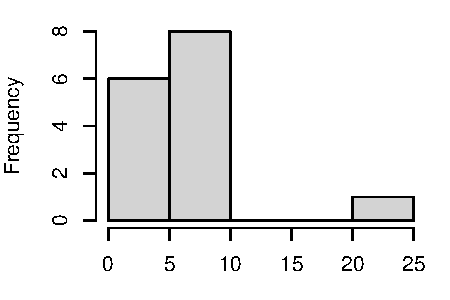
\includegraphics[width=\maxwidth]{figure/unnamed-chunk-1-1} 
\end{knitrout}

\textbf{Exercise 3}.  The following is a histogram of a random sample of $n=200$ observations from a population.  Would it be reasonable to compute a 95\% confidence interval for $\mu$ using this data set?  That is, are the conditions for inference satisfied?

\begin{knitrout}
\definecolor{shadecolor}{rgb}{0.969, 0.969, 0.969}\color{fgcolor}
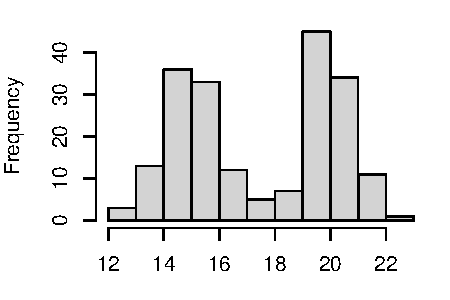
\includegraphics[width=\maxwidth]{figure/unnamed-chunk-2-1} 
\end{knitrout}

\newpage

\textbf{Exercise 4}. [From \emph{OpenIntro} Ch.~7.2]  Let's consider a limited set of climate data,
examining temperature differences in 1948 vs~2018. We sampled 197 locations from the National Oceanic and Atmospheric Administration's (NOAA) historical data, where the data was available for both years of interest. We want to know: were there more days with temperatures exceeding 90$^{\circ}$F in 2018 or in~1948? The difference in number of days exceeding 90$^{\circ}$F (number of days in 2018 - number of days in 1948) was calculated for each of the 197 locations. The average of these differences was 2.9 days with a standard deviation of 17.2 days. We are interested in determining whether these data provide strong evidence that there were more days in 2018 that exceeded 90$^{\circ}$F from NOAA's weather stations.\\
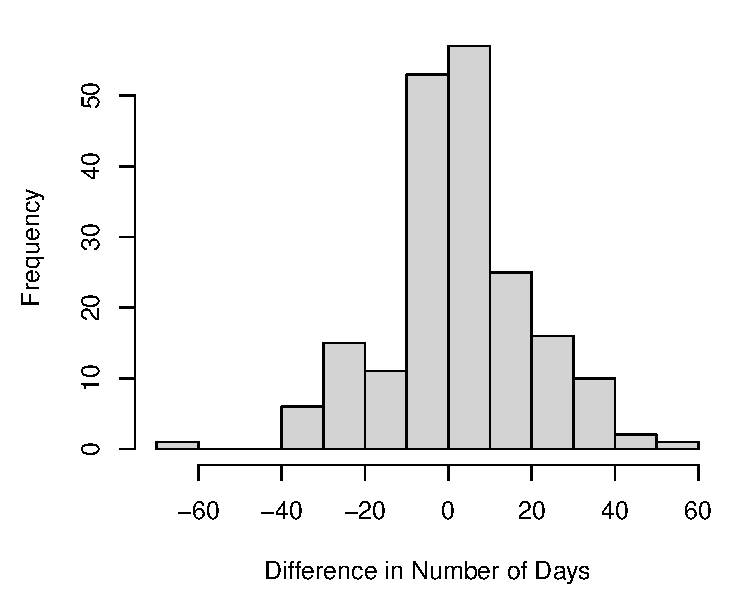
\includegraphics[scale = 0.5]{diff_hist.pdf}

\begin{enumerate}[(a)]
\item Are these data from two independent samples, or are these data paired?
\vspace{1cm}

\item Write the null and alternative hypothesis for a one-sided test.
\vspace{1cm}

\item Are the conditions for the hypothesis test satisfied?
\vspace{3cm}

\item Calculate the test statistic and $p$-value, and make a decision using $\alpha = 0.05$ significance level.\\
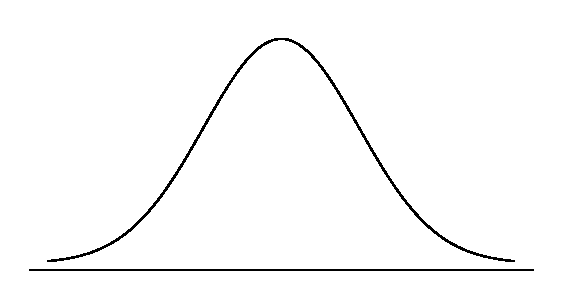
\includegraphics[scale = 0.5]{norm_draw.pdf}

\newpage
\item What is the conclusion of the test in the context of the data?
\vspace{4cm}

\item Calculate and interpret a 90\% confidence interval for the population mean difference between the number of days exceeding 90$^{\circ}$F in 1948 and 2018.\\
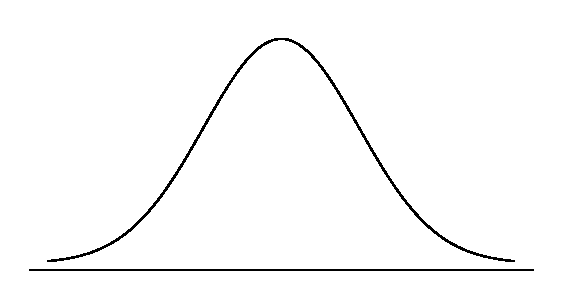
\includegraphics[scale = 0.55]{norm_draw.pdf}
\end{enumerate}




\end{document}
